\section{yEd}
\label{yed}
\prc

Das Programm yEd ist ein Graph Editor, mit dem die verschiedensten Diagrammtypen erstellt werden können. Die Applikation wurde von dem deutschen Unternehmen yWorks entwickelt und basiert auf der Java-Bibliothek yFiles. Dadurch punktet der Editor nicht nur mit den Layout-Algorithmen und den Analyse-Tools die durch die Bibliothek zur verfügung gestellt werden sondern auch mit einem übersichtlichen User-Interface, dass das erstellen und bearbeiten von Diagrammen vereinfacht.
\\

\subsection{Varianten und Installation}

\noindent
Um die Anwendung zu nutzen gibt es zwei Möglichkeiten. Die erste wäre den ,,yEd Live''-Dienst in Anspruch zu nehmen. Dabei handelt es sich um eine Online-Variante. Der Nachteil dieses Services ist, dass die Verarbeitung und auch Darstellung der Daten im Hintergrund anders ist als bei der Offline-Version. Dies führt unter anderem dazu, dass die erzeugten GraphMl-Dateien bei ,,yEd Live'' nicht richtig bis hin zu gar nicht angezeigt werden.
\\

\noindent
Bei der zweiten Methode handelt es sich um die Offline-Version. Diese kann über die offizielle Internetseite von yWorks für das entsprechende Betriebssystem heruntergeladen und danach entsprechend installiert werden.
\\

\noindent
Wichtig ist es bei der Auswahl der Datei für die Installation darauf zu achten, ob diese auch die benötigte Java JRE beinhaltet und wenn nicht, ob man selbst auf dem Rechner die dazugehörige installiert hat. Wenn man sich dann im Installationsprozess befindet kommt man an einen Punkt, an dem man nach einem Installationspfad gefragt wird. Hierbei muss man darauf achten das Programm an einem Ort zu installieren zu dem man als Benutzer auch Zugriff hat, weil das Command-Line-Tool bei der Erstellung eines ER-Diagrammes anbietet, die generierte Grafik, sofern es sich um eine GraphMl Datei handelt und man auf Linux arbeitet, direkt von der Kommandozeile heraus in yEd zu öffnen.

\begin{figure}[!h]
	\begin{center}
		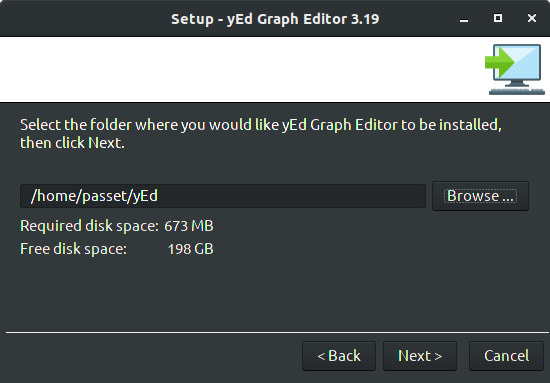
\includegraphics[width=10cm]{images/yed_installation_pfad.png}
		\caption{Angabe des Installationspfades im Installer von yEd 3.19}
		\label{yEdInstaller}
	\end{center}
\end{figure}

\subsection{Oberfläche}
\prc

\noindent
Das grafische Interface mit dem der Benutzer interagiert entspricht zwar nicht den modernsten Design Ideen aber bietet alles was man braucht. Grundlegend kann man die Oberfläche des Editors in 7 Bereiche unterteilen.

\subsubsection{Menü}

Den Kopf der Oberfläche bildet das Menü. Hier kann der Benutzer verschiedene Ansichten und Funktionen aktivieren bzw. deaktivieren. Es umfasst die Menüs Datei, Bearbeiten, Ansicht, Layout, Werkzeuge, Gruppierung, Fenster und Hilfe.

\subsubsection{Palette}

\noindent
In der Palette befinden sich die Elemente mit denen man einen Graphen erstellen kann. Diese Komponenten sind in Gruppen aufgeteilt um für einen besseren Überblick zu sorgen. Zu Beginn bietet der Editor einem die folgenden Gruppierungen mit den entsprechenden Elementen:
\\

\begin{multicols}{2}
    \begin{itemize}
        \item Geometrische Knoten
        \item Moderne Knoten
        \item Kantentypen
        \item Gruppenknoten
        \item Swimlane- und Tabellenknoten
        \item Personen
        \item Computer-Netzwerk
        \item UML
        \item Flussdiagramm
        \item BPMN 
        \item Entity Relationship
        \item SBGN
        \item Aktuelle Elemente
        \\
    \end{itemize}
\end{multicols}

\noindent
Es gibt auch für den Benutzer die Möglichkeit selbst eine Gruppe mit Elementen zu erstellen und diese dann auch in die Palette einzubinden \footfullcite{yEdManual}. 

\begin{figure}[H]
	\begin{center}
		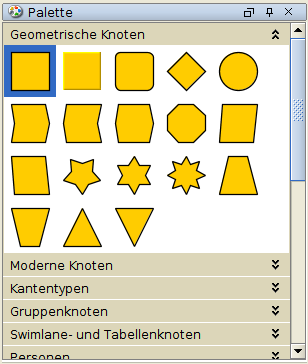
\includegraphics[width=5cm,height=6cm]{images/yed_palette_offen.png}
		\caption{Palette in yEd bei Programmstart}
		\label{yEdPaletteOffen}
	\end{center}
\end{figure}

\subsubsection{Eigenschaften}
\prc

\noindent
Der Bereich Eigenschaften zeigt die charakteristischen Werte des momentan ausgewählten Elementes an. Hier können allerlei verschiedener Veränderungen vorgenommen werden wie zum Beispiel das Ändern der Beschreibung, Größe oder auch Farbe, vorausgesetzt natürlich das diese änderbar sind. Die Merkmale in diesem Bereich werden in die Gruppen Allgemein, Beschriftung, Daten und eine für das Element spezifische Gruppe aufgeteilt. In der Abbildung \ref{yEdEigenschaften} wäre dann die spezifische Gruppe ,,Entity Relationship''.

\begin{figure}[!h]
	\begin{center}
		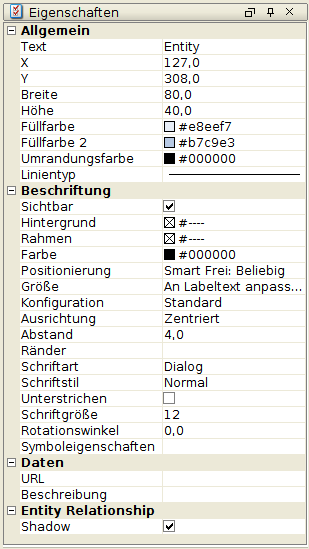
\includegraphics[width=6.5cm,height=10cm]{images/yed_eigenschaften.png}
		\caption{Eigenschaften eines Entitytypen in yEd}
		\label{yEdEigenschaften}
	\end{center}
\end{figure}

\noindent
Sollte man kein Element seines Graphen ausgewählt haben, sieht man in diesem Bereich die Gesamtzahl an Knoten und Kanten. 

\subsubsection{Nachbarschaft}

\noindent
Auf der linken Seite der GUI befinden sich Bereiche die einem Auskunft über den Aufbau des aktuellen Graphen geben. Darunter befindet sich der Bereich Nachbarschaft. In diesem Fenster sieht man demnach alle Nachbar-Knoten des momentan ausgewählten Knoten. Zudem bietet es Registerkarten an, in denen nur die Knoten innerhalb der Gruppe, Vorgänger oder Nachfolger angezeigt werden. 
\\

\noindent
Dies kann sich bei einem Entity-Relationship Diagramm als großen Vorteil entpuppen, da mit einem Klick herausgefunden werden kann mit welchen Beziehungstypen der Entitytyp in relation steht. In der Abbildung \ref{yEdNachbarschaft} wird die Nachbarschaft des Entitytypen Abteilung dargestellt.

\begin{figure}[!h]
	\begin{center}
		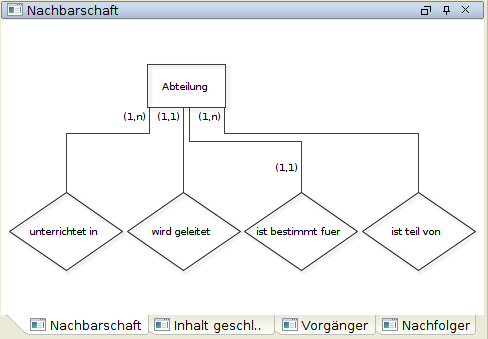
\includegraphics[width=10cm]{images/yed_nachbarschaft.png}
		\caption{Nachbarschaft des Entitytypen Abteilung aus dem Datenmodell Schulinformationssystem}
		\label{yEdNachbarschaft}
	\end{center}
\end{figure}

\subsubsection{Struktur}
\prc
Im wesentlichen beinhaltet dieser Bereich eine Liste mit all den Elementen die sich zum momentanen Zeitpunkt auf der Hauptoberfläche von yEd befinden. Sie ist hierarchisch geordnet, weshalb Teile des Graphen die zuerst erstellt wurden weiter oben angeführt sind als Teile die später hinzugefügt wurden. 
\\

\noindent
Das Fenster Struktur ist eng mit den zuvor genannten Bereichen verbunden. Wählt man eine der Komponenten aus wird sie im Graphen markiert, die Eigenschaften dargestellt und die Nachbarschaft aufgezeigt.

\begin{figure}[H]
	\begin{center}
		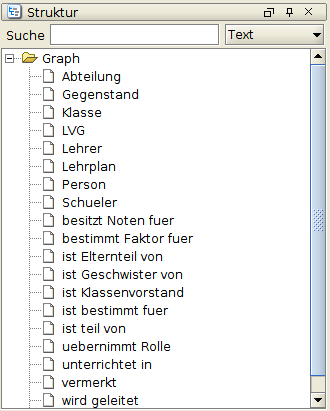
\includegraphics[width=6.5cm,height=7.5cm]{images/yed_struktur.png}
		\caption{Strutkur des ER-Diagrammes Schulinformationssystem}
		\label{yEdStruktur}
	\end{center}
\end{figure}

\subsubsection{Editor-Bereich}
\prc

In diesem Bereich wird der Graph dargestellt und durch Elemente aus der Palette ergänzt und verändert. Dies geschieht durch die Verwendung einer Maus oder durch drücken bestimmter Tasten auf der Tastatur. Die folgenden Aktionen und noch weiter nicht angeführte können auf diese Weise ausgeführt werden:
\\

\begin{itemize}
    \item Einen neuen Knoten erstellen und auswählen
    \item Eine Kante erstellen und auswählen
    \item Knoten verschieben
    \item Eine neuen Biegepunkt auf der Kante erstellen und verschieben
    \item Ein Element löschen
    \item Eine Beschriftung erstellen, auswählen, bearbeiten und verschieben
    \\
\end{itemize}

\noindent
Die folgende Abbildung zeigt einen von yEd generierten Graphen den man ohne weiteres durch die Verwendung der eben genannten Aktionen erstellen kann.

\begin{figure}[H]
	\begin{center}
		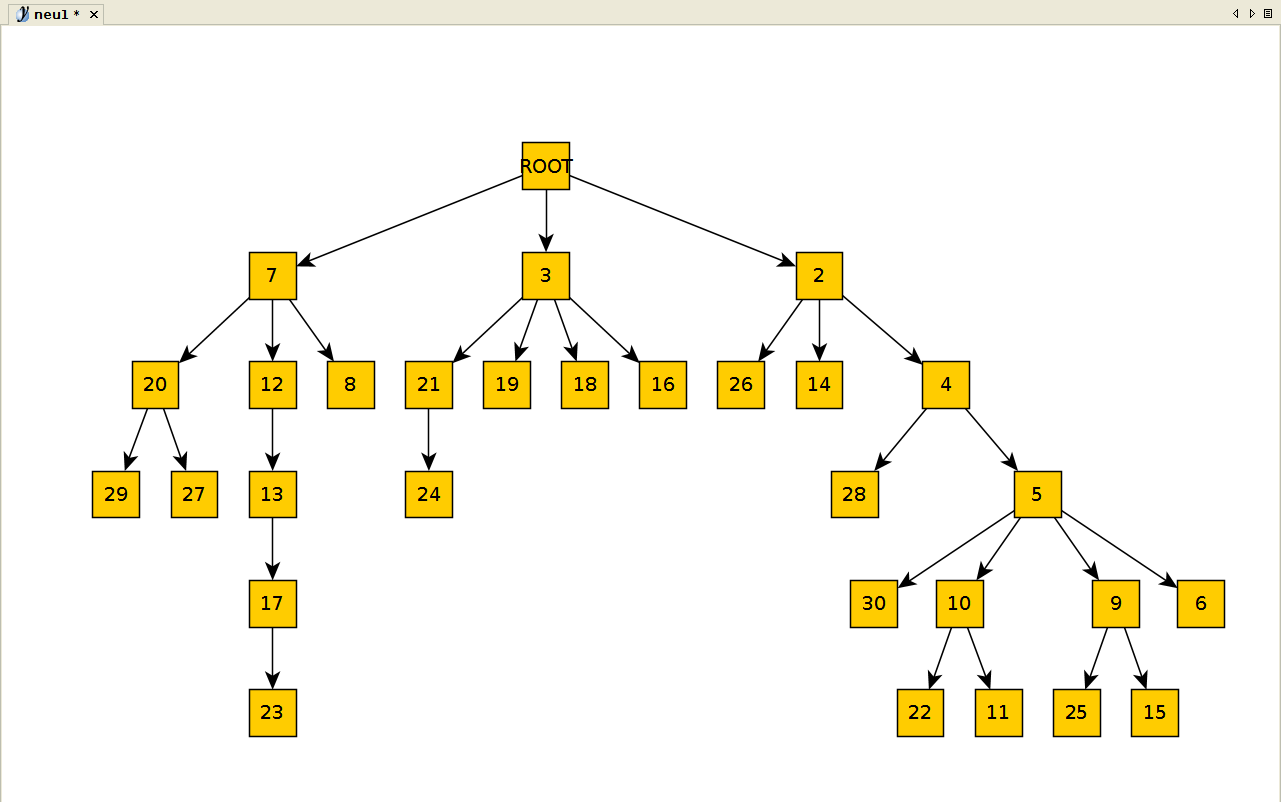
\includegraphics[width=13cm,height=10cm]{images/yed_editor.png}
		\caption{Beispiel Graph generiert von yEd}
		\label{yEdEditor}
	\end{center}
\end{figure}

\subsubsection{Übersicht}

Den letzten Bereich der Oberfläche bietet die Übersicht. Hier wird der gesamte Graph dargestellt. Sollte der Editor-Bereich nicht den ganzen Graphen anzeigen wird in der Übersicht durch eine weiße Form gezeigt was gerade im Editor-Bereich angezeigt wird. Diese Form kann mit dem Mauszeiger durch anklicken und bewegen verschoben werden. Auf diese Weise kann man im Editor-Bereich navigieren.


\subsection{Editier-Hilfen}

Um den Benutzer bei der Anordnung der Elemente seines Graphen zu unterstützen, bietet yEd 3 Features.

\subsubsection{Snap Lines}
\prc
Im \citetitle{yEdManual} wird das Grundkonzept der ,,Snap Lines'' , zu deutsch Hilfslinien, wie folgt beschrieben:

\begin{quote}
    Snap Lines help you to interactively create a graph with an appealing layout.
\end{quote}

\noindent
Zusammenfassend lässt sich also sagen, dass die ,,Snap Lines'' für ein ansprechendes Layout sorgen. Diese Linien werden angezeigt während man ein ausgewähltes Element bewegt. Dabei rastet die Komponente an den Stellen ein wo es gut aussehen könnte und zeigt durch eine Linie an, weshalb es dort eingerastet ist.
\\

\noindent
In der Abbildung \ref{snapLineCenter} sieht man zum Beispiel, dass das ausgewählte Element an dieser Stelle einrastet weil es sich auf der selben Höhe befindet wie das Element das nebenan platziert ist.

\begin{figure}[!h]
	\begin{center}
		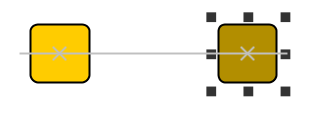
\includegraphics[width=10cm]{images/yed_snap_center.png}
		\caption{,,Snap Line'' hilft bei der zentralen Positionierung}
		\label{snapLineCenter}
	\end{center}
\end{figure}

\noindent
Des Weiteren lassen die ,,Snap Lines'' einen erkennen, ob ein Knoten der zwischen 2 anderen Knoten positioniert wird sich mittig befindet oder ob ein Knoten die selbe Höhe oder Breite hat als ein anderer Knoten.

\subsubsection{Grid}

Eine weitere Hilfestellung für ein gutes Layout ist das Grid, zu deutsch Gitter, das man über die Menüleiste einschalten kann. Hat man es eingeschaltet, rasten die Elemente die man aus der Palette zieht an einem der fest vorgegebenen Punkte ein.

\subsubsection{Orthogonale Kanten}

Das letzte Feature das Abhilfe bei der händischen Anordnung der Komponenten schafft sind die orthogonalen Kanten. Hat man diese Funktion über die Menüleiste von yEd aktiviert, dann werden Kanten nur noch mit 90° Winkeln erstellt. Das heißt, dass es keine schiefen Linien mehr gibt, sondern der Editor von sich aus die Linien horizontal bzw. vertikal zeichnet bis die gewünschten Knoten miteinander verbunden sind, wie in Abbildung \ref{yedOrthogonaleKante} dargestellt wird.

\begin{figure}[H]
	\begin{center}
		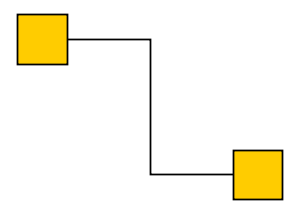
\includegraphics[width=5.5cm]{images/yed_ortogonale_kante.png}
		\caption{Beispiel einer orthogonalen Kante in yEd}
		\label{yedOrthogonaleKante}
	\end{center}
\end{figure}

\subsection{Layout-Algorithmen}
\prc

Einer der größten Vorteile die yEd besitzt, sind die Layout-Algorithmen die der Editor einem zur Verfügung stellt. Insgesamt kann man zwischen 19 verschiedenen auswählen. Diese sind unter anderem: 

\begin{multicols}{2}
	\begin{itemize}
		\item Hierarchisch
		\item Organisch
		\item Orthogonal
		\begin{itemize}
			\item Klassich
			\item UML-Stil
			\item Kompakt
		\end{itemize}
		\item Kreisförmig
		\item Baumartig
		\begin{itemize}
			\item Gerichtet
			\item Ballon
		\end{itemize}
		\item Radial
		\item Serien-Parallel
		\item Swimlane
		\begin{itemize}
			\item Hierarchisch
			\item Organisch
			\item Tabellarisch
		\end{itemize}
		\item Flowchart
		\item BPMN
		\item SBGN
		\item Stammbaum
		\item Tree-Map
		\item One-Click Layout
	\end{itemize}
\end{multicols}

\noindent
Der Benutzer hat natürlich die freie Wahl welches Layout er für sein Diagramm haben möchte aber im \cite{yEdManual} sind Empfehlungen gelistet welcher Algorithmus für welchen Diagrammtyp am besten geeignet ist. In den folgenden Unterkapiteln werden jene Layouts näher beschrieben die für ein ER-Diagramm geeignet sind.

\subsubsection{Orthogonales Layout}

Für Entity-Relationship-Diagramme wird das \textit{Orthogonale Layout} empfohlen. Davon stehen 3 Varianten zur Auswahl:
\\

\begin{itemize}
	\item Klassisch
	\item UML-Stil
	\item Kompakt
	\\
\end{itemize}

\noindent
Jede dieser Methoden verfügt über unterschiedliche Parameter die man als Benutzer festlegen kann und die anschließende Darstellung sichtlich beeinflussen. In der nachfolgenden Abbildung \ref{sisOrthogonalKlassisch} wird ein Beispiel von einem Datenmodell gezeigt, dessen Elemente mithilfe des klassischen Orthagonalen Layout angeordnet wurden.

\begin{figure}[H]
	\begin{center}
		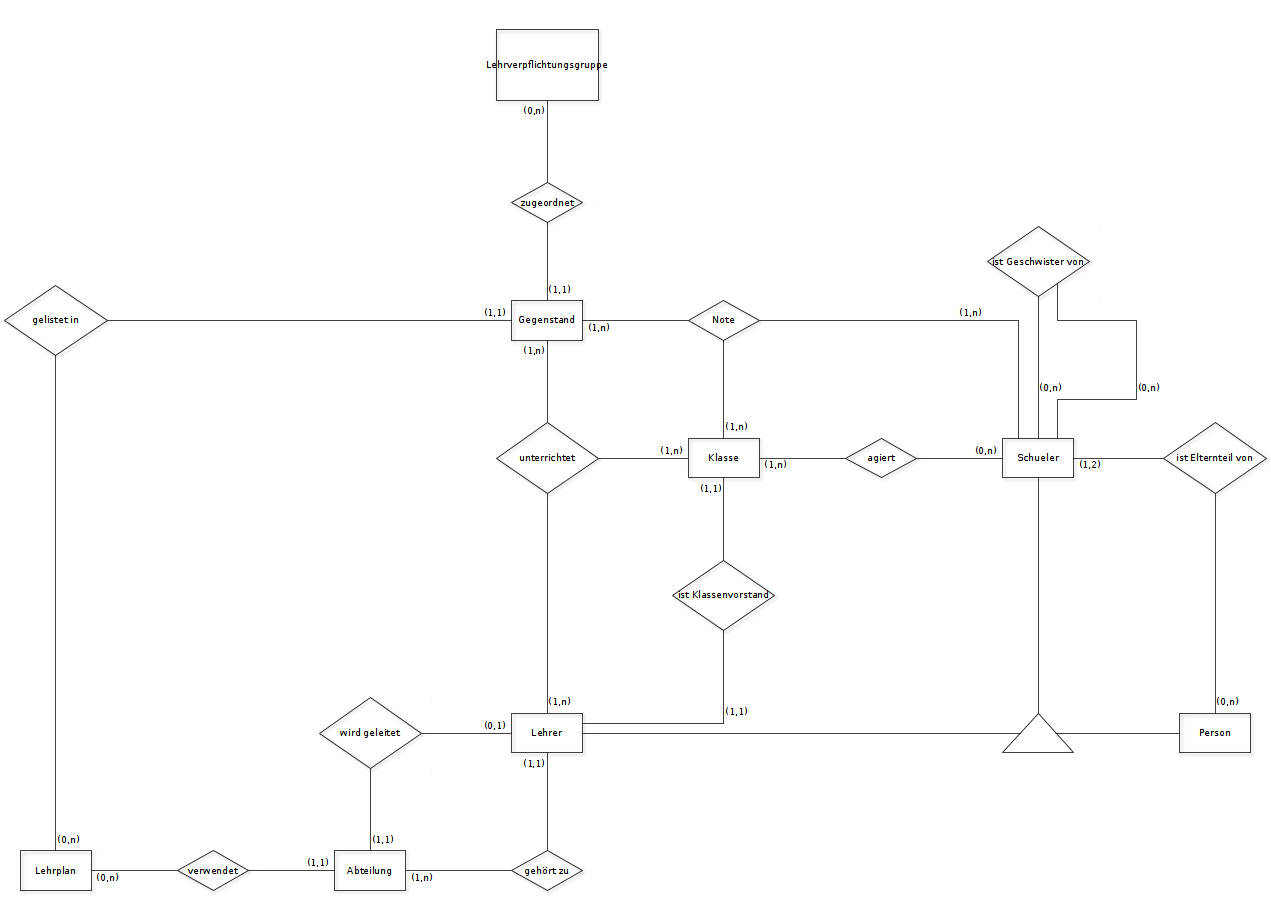
\includegraphics[width=8cm]{images/sisOrthagonal.png}
		\caption{Beispiel für die Anordnung durch klassisches Orthogonales Layout}
		\label{sisOrthogonalKlassisch}
	\end{center}
\end{figure}

\noindent
Wie man sehen kann sind die Kanten alle gerade weshalb es schön anzusehen und auch lesbar ist. Zeichnet man jedoch auch die Attribute in das Diagramm werden wie in Abbildung \ref{orthogonalKlobig} ersichtlich, viele Kanten nah aneinander gelegt, was das Diagramm klobig erscheinen lässt.

\begin{figure}[H]
	\begin{center}
		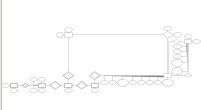
\includegraphics[width=10cm]{images/orthogonalAttribute.png}
		\caption{Orthogonales Layout mit Attributen }
		\label{orthogonalKlobig}
	\end{center}
\end{figure}

\subsubsection{Kreisförmig}
\prc

Im Zuge der Diplomarbeit wurde auch das \textit{Kreisförmige Layout} näher untersucht. Wie der Name schon preisgibt, werden hierbei die Knoten in einem oder mehrere Kreise angeordnet abhängig von den Einstellungen. Bei diesem Layout werden 4 Stile unterschieden:
\\

\begin{itemize}
	\item BCC Kompakt
	\item BCC isoliert
	\item Benutzerdefinierte Gruppen
	\item Einzelner Kreis
\end{itemize}

\noindent
\prc
Für ein ER-Diagramm könnte man die Stile BCC Kompakt und BCC isoliert in betracht ziehen. Bei BCC Kompakt repräsentieren die Teile des Diagramms \textit{biconnected} Komponenten. Diese Komponente wird laut \citetitle{yEdManual} wie folgt definiert:

\begin{quote}
	A biconnected component consists of nodes that are reachable by two edge disjoint paths.
\end{quote}

\noindent
Sollte ein Knoten die Möglichkeit haben zu zwei Komponenten zu gehören wird dieser vom Algorithmus einer Komponente exklusiv zugewiesen.
\\

\noindent
BCC isoliert wendet das selbe verfahren an wie BCC Kompakt. Kommt es hierbei jedoch zu dem Fall, dass ein Knoten zu zwei Komponenten dazugehören könnte wird dieser als eingene Komponente im Diagramm dargestellt \footcite{yEdManual}.
\\

\noindent
Wie man an den Abbildungen \ref{bccKompaktFlug} und \ref{bccIsoliertFlug} erkennen kann, ist es möglich ein ER-Diagramm mit diesem Algorithmus gut darzustellen bzw. es mit wenigen Handgriffen über die Editor-Oberfläche zu verschönern. Jedoch kann sich, abhängig von dem jeweiligen Datenmodell, ein Diagramm wie in Abbildung \ref{bccKompaktSis} entstehen.

\begin{figure}[!h]
	\begin{center}
		\subfigure[Datenmodell Fluggesellschaft mit BCC Kompakt]
		{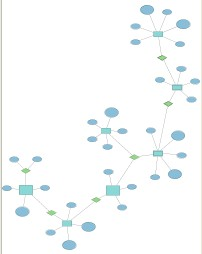
\includegraphics[width=6cm,height=9cm]{images/fluggesellschaftBccKompakt.png}
		\label{bccKompaktFlug}}
		\subfigure[Datenmodell Fluggesellschaft mit BCC isoliert]
		{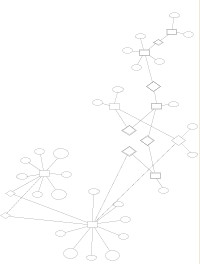
\includegraphics[width=6cm,height=9cm]{images/fluggesellschaftBccIsoliert.png}
		\label{bccIsoliertFlug}}
	\caption{Datenmodell Fluggesellschaft in BCC Kompakt und BCC isoliert}
	\end{center}
\end{figure}

\begin{figure}[!h]
	\begin{center}
		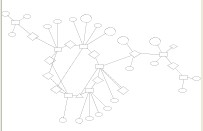
\includegraphics[width=8cm]{images/sisBccKompakt.png}
		\caption{Datenmodell Schulinformationssystem mit BCC Kompakt}
		\label{bccKompaktSis}
	\end{center}
\end{figure}

